%  CONFIGURE NEW SINGLE-PAGE FORMAT 

\onecolumn % go back to one column
\fancyhead{} % make sure we get no headers
\renewcommand{\floatpagefraction}{0.1}
\lfoot[\bSupInf]{\dAuthor}
\rfoot[\dAuthor]{\cSupInf}
\newpage

\captionsetup*{format=largeformat} % make figure legend slightly larger than in the paper
\setcounter{figure}{0} % reset figure counter for Supp. Figures
\setcounter{equation}{0} % reset equation counter for Supp. Equations
%\setcounter{page}{1} % reset page count
\makeatletter 
\renewcommand{\thefigure}{S\@arabic\c@figure} % make Figure legend start with Figure S
\makeatother
\def\theequation{S\arabic{equation}}

%  MAIN TEXT 

\newpage
\section*{Supplementary Information}

%--------------------------------------------------------------------
\subsection*{Appendix 1 - Patch Weight Distributional Assumptions}\label{app:app-1}
%--------------------------------------------------------------------

\subsubsection*{Theoretical Justification}

We make a simplifying assumption regarding path weights where we assume that patch occupancy probabilities are uniformly distributed on the interval $(0,2/n)$, and that for large enough $n$ their sum converges to 1 (satisfying their use as weights). To show briefly that this assumption is valid, we walk through what this means. 

Suppose patch weights are independently drawn from a uniform distribution:
\begin{equation}
w_i \sim \text{Uniform}\left(0, \frac{2}{n}\right), \quad i = 1, \dots, n.
\end{equation}

Then for each weight it follows that the expected value and the variance would be:
\begin{align}
     \mathbb{E}[w_i] &=  \frac{1}{n}\\
     \text{Var}(w_i) &= \frac{1}{12} \left(\frac{2}{n} - 0\right)^2 \\
     &=  \frac{1}{3n^2}
\end{align}


The sum of the weights is:
\begin{equation}
\zeta_n = \sum_{i=1}^{n} w_i,
\end{equation}
with expected value:
\begin{equation}
\mathbb{E}[\zeta_n] = \sum_{i=1}^{n} \mathbb{E}[w_i] = n \cdot \frac{1}{n} = 1,
\end{equation}
and variance:
\begin{equation}
\text{Var}(\zeta_n) = \sum_{i=1}^{n} \text{Var}(w_i) = n \cdot \frac{1}{3n^2} = \frac{1}{3n}.
\end{equation}

Therefore, as \( n \to \infty \),
\begin{equation}
\mathbb{E}[\zeta_n] \to 1 \quad \text{and} \quad \text{Var}(\zeta_n) \to 0,
\end{equation}
which implies that the sum of unnormalized weights converges in probability to 1:
\begin{equation}
\zeta_n \xrightarrow{P} 1.
\end{equation}

\subsubsection*{Simulations}

We show that this holds in a simulated environment for two cases, uniform random weights and uniform random weights with some variance $q$. To do this, we compare the cases where $w$ is given by constant weights, and where $w \approx  \mathcal{U}(1/n-q,1/n+q)$. Since the expected value of $\zeta_n$ is 1, we simulated across a variety of numbers of $n$, drawing weights $w$ in either of the two ways above 1000 times, and then calculated the average squared deviation and the average absolute deviation via 

\begin{equation}
    \begin{aligned}
    \text{dev}_{\text{sq}} &= \left( \sum_{i=1}^n w_i - 1\right) ^ 2 \\ 
    \text{dev}_{\text{abs}} &= \left| \sum_{i=1}^n w_i - 1\right|
    \end{aligned}
    \label{eq:dev-measures}
\end{equation}

We simulated across values of $n$ from 1,000 to 10,000,000. In both cases (with and without $q$, we show that both measures of deviation converge to $0$ at large numbers of $n$ (\Cref{fig:patch-weight-abs,fig:patch-weight-sq}). In the case of no variance, as expected, the values of both measures of deviance are $\sim 0$ for all values of $n$. To balance both computational efficiency as well as satisfying the exceptions and assumptions outlined here, we thus chose a number of patches, $n = 200,000$ as being sufficient to capture the dynamics of the system. 

\begin{figure}[!hpt]
    \centering
    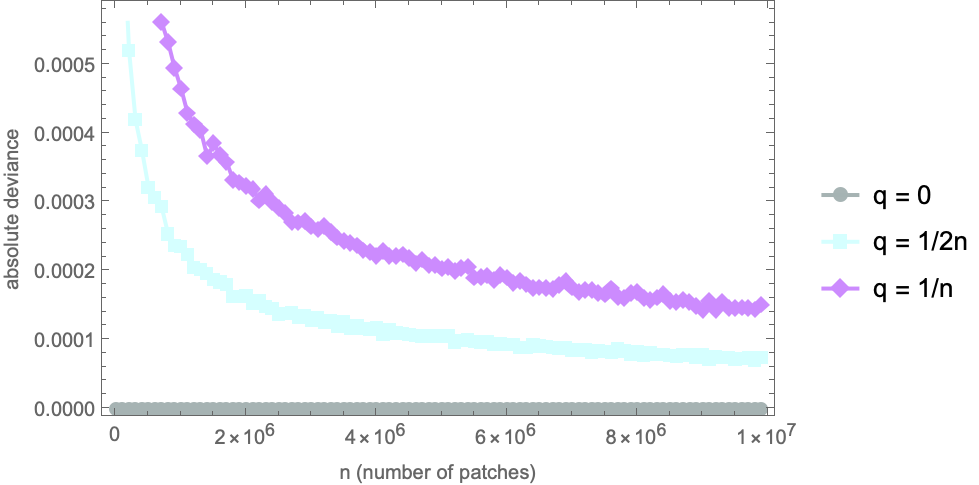
\includegraphics[width=0.8\linewidth]{figs/si/patch-weight-convergence/absPlotAll.png}
    \caption{Absolute deviance as measured by \cref{eq:dev-measures}, versus the number of patches in the landscape. Each point represents the mean value from 1,000 random draws of $w$ for a given $n$ and $q$. This represents the case where $w$ is drawn from a uniform random distribution with no variance (i.e. $q=0$), maximum variance ($q=1/n$) and medium variance ($q=1/2n$}). 
    \label{fig:patch-weight-abs}
\end{figure}
\begin{figure}[!hpt]
    \centering
    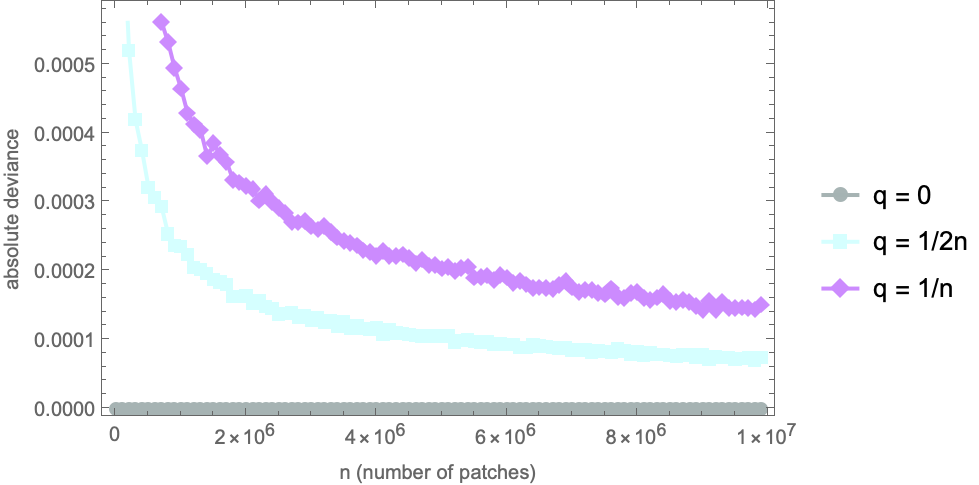
\includegraphics[width=0.8\linewidth]{figs/si/patch-weight-convergence/absPlotAll.png}
    \caption{Squared deviance as measured by \cref{eq:dev-measures}, versus the number of patches in the landscape. Each point represents the mean value from 1,000 random draws of $w$ for a given $n$ and $q$. This represents the case where $w$ is drawn from a uniform random distribution with no variance (i.e. $q=0$), maximum variance ($q=1/n$) and medium variance ($q=1/2n$)}. 
    \label{fig:patch-weight-sq}
\end{figure}
\newpage

%--------------------------------------------------------------------
\subsection*{Appendix 2 - Simulation strategies for landscape--level contagion (\texttt{\color{blue}r0-simulations.nb})}\label{app:app-2}
%--------------------------------------------------------------------

We consider two distinct inferential targets and, accordingly, adopt two computational strategies of very different complexity.  Table \ref{tab:sim_overview} summarises the mapping between \emph{question}, \emph{assumptions}, \emph{Mathematica implementation}, and \emph{computational cost}.

%--------------------------------------------------------------------
\paragraph{(A) Uniform--weight epidemic trajectories.}\mbox{}\\

The first question is: \begin{quote} \textit{“Given a landscape with $n$ patches of equal attractiveness ($w_j \equiv 1/n$), what is the distribution of outbreak metrics such as extinction time, epidemic size, and prevalence through time?”} \end{quote}

\noindent
Because all patches are exchangeable, the state of the system at time $t$ is fully described by the \emph{number of infected individuals} $\,I_t\,$.  The per--step infection probability for a given susceptible is
\begin{equation}
  p_t \;=\;
  1-\!\left(1-\frac1n\right)^{I_t}
  \;\approx\;
  1-\exp\!\Bigl(-\tfrac{I_t}{n}\Bigr),
  \label{eq:pt_uniform}
\end{equation}
so that the update
\begin{equation}
  I_{t+1} \;\sim\;
  \text{Binomial}\!\bigl(N_T-I_t,\;p_t\bigr)
  \label{eq:binom_update}
\end{equation}
is $\mathcal O(1)$ regardless of population size.%
\footnote{%
$N_T$ denotes the fixed census size
$N_T=S+I_t$}
Function \texttt{\color{blue}simulateRunFast} implements
\eqref{eq:binom_update}; its sparse
counterpart \texttt{\color{blue}simulateRunSparse} retains explicit patch indices for later spatial analyses at the expense of a mild speed penalty.

%--------------------------------------------------------------------
\paragraph{(B) Heterogeneous--weight basic reproduction number.}\mbox{}\\

The second question, addressed in the $q$–sweep, is: \begin{quote} \textit{“How does patch--level heterogeneity, controlled by $w_j \sim \text{U}(1/n-q,\,1/n+q)$, inflate the landscape-level basic reproduction number $R_0(q)$?”} \end{quote}

\noindent
Here we require only the \emph{first generation} of infection started by a single index case.  Let $w_I$ be the weight of the patch chosen by that index case. Given $S$ susceptibles, the offspring distribution is
\begin{equation}
  I_1 \;\sim\; \text{Binomial}\!\bigl(S,\,w_I\bigr),
  \label{eq:binom_firstgen}
\end{equation}
and the theoretical expectation satisfies%
\footnote{%
Proof follows the derivation in \cref{app:r0_heterogeneity}.}
\begin{equation}
  \mathbb E[I_1]
  \;=\;
  \frac{S}{n}
  \;+\;
  \frac{n\,S\,q^{2}}{3}.
  \label{eq:r0_theory}
\end{equation}

Two implementations are provided:

\begin{itemize}
\item
\texttt{\color{blue}simulateR0FastSameWeights}:\ draws a \emph{single} weight vector for each $q$ and performs all $\texttt{numReps}$ replicates on that fixed landscape (vectorised calls to \texttt{RandomVariate}).
\item
\texttt{\color{blue}simulateR0FastFreshWeights}:\ regenerates weights every replicate; still $\mathcal O(1)$ per replicate because only $w_I$ and one binomial variate are required.
\end{itemize}

%--------------------------------------------------------------------
\paragraph{Trade–offs and compatibility.}\mbox{}\\

\begin{itemize}
\item  Strategy~(A) captures \emph{multi–generation dynamics}
      but assumes strictly uniform weights
      [$w_j\equiv 1/n$, cf.\ \eqref{eq:pt_uniform}].
\item  Strategy~(B) quantifies the \emph{initial} amplification of
      transmission caused by heterogeneity
      [Eq.~\eqref{eq:r0_theory}] but does not model the temporal feedback
      of weight variability beyond the first step.
\item  The two strategies are therefore complementary rather than
      contradictory: they target different summary statistics of the
      \emph{same} underlying model. Using them in tandem is logically
      consistent provided results from (B) are interpreted strictly as
      $R_0(q)$ estimates and not as full epidemic forecasts.
\item  Computationally, (A) scales with the time horizon and would be
      prohibitive under heterogeneous weights unless additional summary
      statistics of the infected–patch weight distribution were tracked.
      Strategy~(B) is embarrassingly parallel and completes in
      seconds even for \texttt{numReps}$\ge 10^{5}$.
\end{itemize}

%--------------------------------------------------------------------
\begin{table}[t]
  \centering
  \footnotesize
  \caption{Overview of simulation styles.\label{tab:sim_overview}}
  \begin{tabular}{@{}p{3cm}p{3.5cm}p{4.0cm}p{3.8cm}@{}}
    \toprule
    \textbf{Question} &
    \textbf{Key assumption} &
    \textbf{Mathematica function(s)} &
    \textbf{Computational cost per replicate} \\ \midrule
    Trajectory\newline metrics &
    Uniform weights &
    \texttt{simulateRunFast}\newline
    (\texttt{simulateRunSparse} if patch IDs needed) &
    $\mathcal O(1)$ per time step\newline
    $\mathcal O$(\texttt{maxTime}) total \\[0.6em]
    $R_0(q)$ sweep &
    Heterogeneous $\text{U}(1/n\!\mp\!q)$ weights,
    single generation &
    \texttt{simulateR0FastSameWeights}\newline
    or \texttt{simulateR0FastFreshWeights} &
    $\mathcal O(1)$ (one binomial draw) \\ \bottomrule
  \end{tabular}
\end{table}

%======================================================================
\subsection*{Derivation of the heterogeneous-weight reproduction number}%
\label{sec:r0_heterogeneity}
%======================================================================

We establish the closed–form expression
\begin{equation}
  \boxed{\;
    \mathbb{E}\!\bigl[I_{1}\bigr]
      \;=\;
      \frac{S}{n}
      \;+\;
      \frac{n\,S\,q^{2}}{3}
  \;}
  \label{eq:r0_app_goal}
\end{equation}
for the expected number of first–generation infections $I_{1}$ produced
by a single index case on a landscape of $n$ patches whose relative
attractiveness's (``weights'') are perturbed from perfect uniformity by a
tunable parameter $q$.

%----------------------------------------------------------------------
\subsubsection*{Weight-sampling scheme}
%----------------------------------------------------------------------

\begin{enumerate}
\item \textbf{Raw weights.}  
  Draw independent%
  \footnote{Independence is the strongest assumption used;
            mild correlations do not change the leading
            $q^{2}$ behaviour.} raw weights
  $
    x_{j}\;\sim\; \operatorname{U}(n^{-1}-q,\;n^{-1}+q),
    \quad j=1,\dots,n,
  $
  where $0 \le q < n^{-1}$ guarantees positivity.

\item \textbf{Normalization.}  
  The realized patch weights are
  \begin{equation}
    w_{j}
      \;=\;
      \frac{x_{j}}
           {\displaystyle\sum_{k=1}^{n} x_{k}},
    \qquad j=1,\dots,n,
    \label{eq:w_normalise}
  \end{equation}
  so that $\sum_{j} w_{j}=1$ by construction.
\end{enumerate}

%----------------------------------------------------------------------
\subsubsection*{Index-patch weight as a quadratic form}
%----------------------------------------------------------------------

Let $J$ be the random patch chosen by the index case, with
$\Pr[J=j]=w_{j}$.  Define
$
  w_{I} := w_{J}
$
(the subscript $I$ denotes the \textit{I}ndex infected).  Then
\begin{equation}
  \mathbb{E}[w_{I}]
    \;=\;
    \sum_{j=1}^{n} \mathbb{E}[w_{j}^{2}],
    \label{eq:EwI}
\end{equation}
because 
\begin{equation}
\mathbb{E}[w_{J}]
      =\sum_{j} \Pr[J=j]\,w_{j}
      =\sum_{j} w_{j}^{2}.
\end{equation}

With $S$ susceptibles and a single infectious individual, the offspring
distribution is binomial:
\begin{equation}
  I_{1}\;\bigl|\;w_{I} \;\sim\;
    \operatorname{Binomial}(S,\,w_{I}),
  \label{eq:I1_binom}
\end{equation}
so taking expectations of \eqref{eq:I1_binom} and inserting
\eqref{eq:EwI} yields
\begin{equation}
  \mathbb{E}[I_{1}]
    \;=\; S \,\sum_{j=1}^{n} \mathbb{E}[w_{j}^{2}].
  \label{eq:EI1_sumwj2}
\end{equation}

%----------------------------------------------------------------------
\subsubsection*{Moment of a normalized uniform variate}
%----------------------------------------------------------------------

Write $\mu_{x}$ and $\sigma_{x}^{2}$ for the mean and variance of the
uniform raw weight:
\[
  \mu_{x} = \frac{1}{n}, 
  \qquad
  \sigma_{x}^{2} = \frac{q^{2}}{3}.
\]

Denote the raw–weight sum by $T := \sum_{k} x_{k}$.  By the Law of Large Numbers, $T = n\mu_{x}+O_{\mathbb{P}}(n^{1/2})$, so for large $n$
\begin{equation}
  \tfrac1T = \frac{1}{n\mu_{x}}
             + O_{\mathbb{P}}\!\bigl(n^{-3/2}\bigr)
           = 1 + O_{\mathbb{P}}\!\bigl(n^{-1/2}\bigr).
\end{equation}
Retaining terms up to $O(q^{2})$ and $O(n^{-1})$ we therefore have
\begin{align}
  \mathbb{E}[w_{j}^{2}]
    &= \mathbb{E}\!\Bigl[\,x_{j}^{2}\,T^{-2}\Bigr]
      \;\approx\;
      \mathbb{E}[x_{j}^{2}]
      \notag\\
    &= \mu_{x}^{2} + \sigma_{x}^{2}
      \;=\;
      \frac{1}{n^{2}} \;+\; \frac{q^{2}}{3}.
      \label{eq:wj2_moment}
\end{align}

%----------------------------------------------------------------------
\subsubsection*{Summation and final expression}
%----------------------------------------------------------------------

Insert \eqref{eq:wj2_moment} into
\eqref{eq:EI1_sumwj2}:
\begin{equation}
  \mathbb{E}[I_{1}]
    = S
      \left(
        n\!\left[\frac{1}{n^{2}} + \frac{q^{2}}{3}\right]
      \right)
    = 
      \frac{S}{n} \;+\; \frac{n\,S\,q^{2}}{3},
\end{equation}
which is exactly \eqref{eq:r0_app_goal}.  \hfill$\square$

%======================================================================
\subsection{Empirical checks against simulation output}%
\label{app:figures}
%======================================================================

We successfully illustrated how the simulation strategies of \cref{app:app-2} reproduce the qualitative behavior anticipated from the analytic theory derived above.

%----------------------------------------------------------------------
\begin{figure}[h]
  \centering
  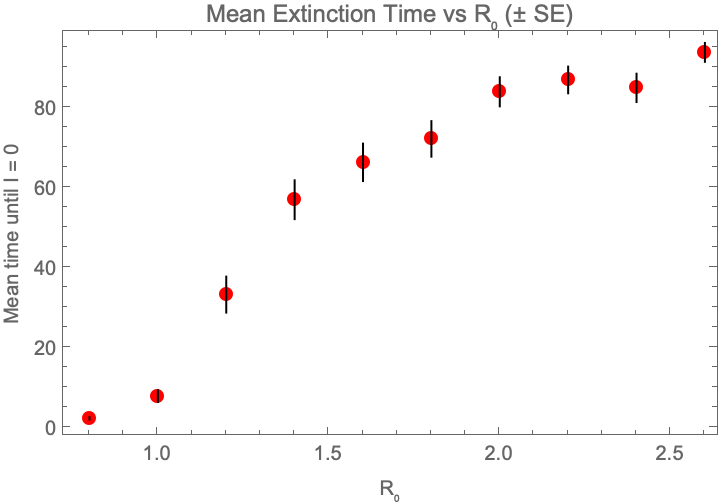
\includegraphics[width=0.85\textwidth]{figs/si/r0-simulations/extinction-time-vs-r0.png}%
  \caption{Mean extinction time (±\,SE) as a function of the basic reproduction number $R_{0}$ under \emph{uniform} patch weights. Each point aggregates 1000 realisations generated with a horizon of 1000. Consistent with branching-process intuition, the mean time to extinction increases sharply as soon as $R_{0}$ exceeds unity and then saturates for $R_{0}\gtrsim 2.5$. These results validate that the uniform-weight epidemic simulator correctly captures the expected critical transition around $R_{0}=1$.}
  \label{fig:extinction_vs_r0}
\end{figure}

%----------------------------------------------------------------------
\begin{figure}[h]
  \centering
  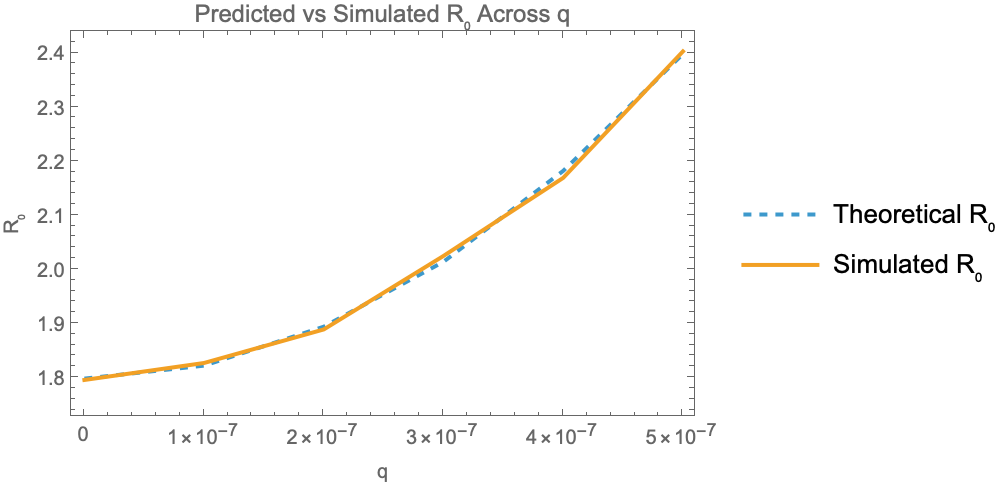
\includegraphics[width=0.85\textwidth]{figs/si/r0-simulations/predicted-vs-simulated-r0-with-q.png}%
  \caption{Comparison between the theoretical prediction \eqref{eq:r0_app_goal} (dashed blue line) and the simulated mean obtained across a geometric sequence of heterogeneity parameters $q$. Simulation settings: \texttt{n}~=~$2e^6$ patches and 10\,000 replicates per $q$. The excellent overlap confirms that \eqref{eq:r0_app_goal} captures the leading $q^{2}/3$ increase in $R_{0}$ predicted by the moment calculation of \ref{sec:r0_heterogeneity}.}
  \label{fig:pred_vs_sim_r0}
\end{figure}

\medskip
Taken together, \cref{fig:extinction_vs_r0,fig:pred_vs_sim_r0} demonstrate that the uniform weightw, multi-generation dynamics and heterogeneous weights, single-generation $R_{0}$ sweep faithfully reproduce the theoretical behavior expected under their respective modeling assumptions.
